\documentclass[12pt,a4paper]{article}
\usepackage[UTF8]{ctex}
\usepackage{amsmath}
\usepackage{graphicx}
\usepackage{booktabs}
\usepackage{geometry}
\usepackage{ulem}
\usepackage{array}
\graphicspath{{e:/USTC/课程/大物实验/核磁共振-徐子钦/}{./}}
\geometry{left=2.5cm,right=2.5cm,top=2.5cm,bottom=2.5cm}

\title{\Huge{\textbf{核磁共振实验报告}}}
\author{\parbox{0.9\textwidth}{\centering 学院：\uline{少年班学院}\\ 姓名：\uline{徐子钦}\\ 学号：\uline{PB24000224}\\ 年级：\uline{24级少院}\\ 日期：\uline{2026.5.1}}}

\begin{document}
\maketitle

\begin{abstract}
本实验采用稳态吸收法研究核磁共振现象。根据 $^1\mathrm{H}$ 与 $^{19}\mathrm{F}$ 样品的共振频率，结合已知静磁场强度计算了两种核的旋磁比与 $g$ 因子；同时通过不同磁场位置的测量考察了磁场均匀性，并利用相邻共振峰频率差估算了调制磁场幅值。实验记录表明，$^1\mathrm{H}$ 的平均共振频率为 $20.6934\,\mathrm{MHz}$，$^{19}\mathrm{F}$ 的平均共振频率为 $19.4633\,\mathrm{MHz}$，对应的 $g$ 因子分别为 $5.62$ 和 $5.29$，与标准值符合较好。

\textbf{关键词}：核磁共振；旋磁比；$g$ 因子；磁场均匀性；调制磁场
\end{abstract}

\section{实验目的}
\begin{enumerate}
    \item 观察核磁共振稳态吸收信号，理解共振条件与磁场、频率之间的关系。
    \item 测量 $^1\mathrm{H}$ 和 $^{19}\mathrm{F}$ 的共振频率，计算对应的旋磁比 $\gamma$ 和 $g$ 因子。
    \item 通过不同位置的测量，考察静磁场 $B_0$ 的空间均匀性。
    \item 利用共振峰间距数据估算调制磁场幅值 $B_m$，加深对扫场法工作机理的理解。
\end{enumerate}

\section{实验原理}
核磁共振是具有磁矩的原子核在恒定磁场 $B_0$ 中发生的能级跃迁现象。原子核具有自旋角动量，因此也伴随有磁矩；当它置于外磁场中时，磁矩不再取任意取向，而是沿磁场方向发生量子化取向。对于自旋 $1/2$ 的原子核，其能级分裂满足
\[
\Delta E = h\nu = \gamma \hbar B_0 = g\mu_N B_0,
\]
其中 $\nu$ 为共振频率，$\gamma$ 为旋磁比，$\mu_N$ 为核磁子，$g$ 为核 $g$ 因子。由此可得
\[
\gamma = \frac{2\pi\nu}{B_0}, \qquad g = \frac{\gamma\hbar}{\mu_N} = \frac{h\nu}{\mu_N B_0}.
\]

从经典图像看，原子核磁矩在静磁场中会绕磁场方向以拉莫尔角频率进动；从量子图像看，磁矩的两个取向对应两条塞曼能级，二者间的能量差由 $B_0$ 决定。当射频场频率与拉莫尔频率一致时，核系统吸收电磁波能量并发生跃迁，示波器上便可观察到共振吸收信号。由于室温下两能级粒子数差很小，共振信号通常较弱，因此实验中必须保证磁场足够稳定且均匀，并借助调制磁场把共振点“扫”出来。

实验采用稳态吸收法：在静磁场 $B_0$ 上叠加低频调制场 $B_m\cos\omega t$，使样品处总磁场在共振条件附近周期性扫过。这样一来，即使射频频率保持近似不变，样品所处的瞬时磁场也会随时间变化，从而使吸收峰在示波器上表现为一个周期性的共振波包或峰列。当射频场频率满足
\[
h\nu = \Delta E,
\]
即可在示波器上观察到共振信号。若相邻共振峰对应的频率差为 $\Delta\nu$，则调制磁场幅值可由
\[
B_m = \frac{2\pi\Delta\nu}{\gamma}
\]
求得。

实验中分别选取 $^1\mathrm{H}$ 与 $^{19}\mathrm{F}$ 样品，是因为它们都具有较强的核磁响应且 $g$ 因子和旋磁比较为典型，适合用来检验核磁共振条件。通过对不同样品共振频率的测量，可以反向求得静磁场强度，也可以进一步比较不同原子核的磁学性质。

\section{实验数据与处理}
\subsection{实验器材}
本实验主要使用以下器材：边限振荡器、永久磁铁、扫场线圈、示波器、频率计以及 $^1\mathrm{H}$ 和 $^{19}\mathrm{F}$ 样品。实验过程中通过边限振荡器提供射频场，通过扫场线圈叠加低频调制场，并利用示波器观察共振信号形状与峰位变化。

\subsection{实验条件}
实验记录中的静磁场取 $B_0 = 483\,\mathrm{mT}$。该数值由样品共振频率与已知核参数反推得到，是后续 $\gamma$ 和 $g$ 因子计算的基础。

\subsection{$^1\mathrm{H}$ 样品共振频率与 $g$ 因子}
\begin{table}[htbp]
\centering
\caption{$^1\mathrm{H}$ 样品共振频率测量数据}
\begin{tabular}{ccccccc}
\toprule
测量次数 & 1 & 2 & 3 & 4 & 5 & 6 \\
\midrule
$\nu$/MHz & 20.6934 & 20.6938 & 20.6929 & 20.6935 & 20.6937 & 20.6932 \\
\bottomrule
\end{tabular}
\end{table}

\[
\bar{\nu}_{\mathrm{H}} = 20.6934\,\mathrm{MHz}
\]

由 $\gamma = 2\pi\bar{\nu}/B_0$ 得
\[
\gamma_{\mathrm{H}} = \frac{2\pi\times 20.6934\times 10^6}{0.483}
= 2.692\times 10^8\,\mathrm{rad\cdot s^{-1}\cdot T^{-1}}.
\]
再由 $g = \gamma\hbar/\mu_N$ 得
\[
g_{\mathrm{H}} = 5.62.
\]

\subsection{$^{19}\mathrm{F}$ 样品共振频率与 $g$ 因子}
\begin{table}[htbp]
\centering
\caption{$^{19}\mathrm{F}$ 样品共振频率测量数据}
\begin{tabular}{ccccccc}
\toprule
测量次数 & 1 & 2 & 3 & 4 & 5 & 6 \\
\midrule
$\nu$/MHz & 19.4632 & 19.4635 & 19.4623 & 19.4642 & 19.4629 & 19.4639 \\
\bottomrule
\end{tabular}
\end{table}

\[
\bar{\nu}_{\mathrm{F}} = 19.4633\,\mathrm{MHz}
\]

由 $\gamma = 2\pi\bar{\nu}/B_0$ 得
\[
\gamma_{\mathrm{F}} = \frac{2\pi\times 19.4633\times 10^6}{0.483}
= 2.532\times 10^8\,\mathrm{rad\cdot s^{-1}\cdot T^{-1}}.
\]
再由 $g = \gamma\hbar/\mu_N$ 得
\[
g_{\mathrm{F}} = 5.29.
\]

\subsection{不同位置的磁场测量}
\begin{table}[htbp]
\centering
\caption{不同位置处的静磁场测量结果}
\begin{tabular}{ccccc}
\toprule
位置/cm & 1 & 2 & 3 & 4 \\
\midrule
$\nu$/MHz & 20.6927 & 20.6925 & 20.6897 & 20.6829 \\
$B$/mT & 482.97 & 482.97 & 482.90 & 482.74 \\
\bottomrule
\end{tabular}
\end{table}

不同位置下磁感应强度的平均值为
\[
\bar{B} = 482.90\,\mathrm{mT}.
\]
测量结果表明，样品所在区域的静磁场较稳定，但仍存在小幅空间变化。

\subsection{调制磁场幅值测量方法与数据}
\paragraph{测量方法（简述）}
在扫场观测中，共振峰列会随射频频率的微调发生如下演化：
\[
\text{出现}\;\rightarrow\;\text{峰间距增大}\;\rightarrow\;\text{峰间距相等（严格共振）}\;\rightarrow\;\text{峰间距减小}\;\rightarrow\;\text{消失}.
\]
据此可通过示波器峰列形态定位两种特殊状态，并读出频率计示值：
\begin{enumerate}
    \item 峰列呈等间距时，记频率为 $\nu_{\mathrm{eq}}$。该情形近似对应调制场取 $B=0$。
    \item 继续微调直至峰列刚好消失时，记频率为 $\nu_{\mathrm{dis}}$。该情形可近似看作调制场瞬时达到最大值 $B=B_m$。
\end{enumerate}
于是两种情形的频率差
\[
\Delta f = \nu_{\mathrm{dis}}-\nu_{\mathrm{eq}}
\]
对应的磁场差恰为 $B_m$。由共振关系 $\nu=\gamma B/2\pi$ 得
\[
\Delta f = \frac{\gamma}{2\pi} B_m \quad\Longrightarrow\quad B_m = \frac{2\pi\Delta f}{\gamma}.
\]
因此测出 $\Delta f$ 并代入已知的 $\gamma$ 即可求得调制磁场幅值 $B_m$。

\paragraph{测量数据}
\begin{table}[htbp]
\centering
\caption{调制磁场幅值测量数据}
\begin{tabular}{ccccccc}
\toprule
测量次数 & 1 & 2 & 3 & 4 & 5 & 6 \\
\midrule
$\nu_{\mathrm{dis}}$/MHz & 20.7006 & 20.7008 & 20.7012 & 20.7002 & 20.7003 & 20.7001 \\
$\nu_{\mathrm{eq}}$/MHz & 20.6937 & 20.6932 & 20.6929 & 20.6938 & 20.6933 & 20.6933 \\
$\Delta f$/MHz & 0.0069 & 0.0076 & 0.0081 & 0.0064 & 0.0070 & 0.0068 \\
\bottomrule
\end{tabular}
\end{table}

\[
\overline{\Delta f} = 0.0071\,\mathrm{MHz}
\]

根据上式计算得
\[
B_m = 0.1657\,\mathrm{mT}.
\]

\section{结果与讨论}
本实验的结果可以概括为以下四点。
\begin{enumerate}
    \item $^1\mathrm{H}$ 样品的平均共振频率为 $20.6934\,\mathrm{MHz}$，对应 $\gamma_{\mathrm{H}} = 2.692\times 10^8\,\mathrm{rad\cdot s^{-1}\cdot T^{-1}}$，$g_{\mathrm{H}} = 5.62$。
    \item $^{19}\mathrm{F}$ 样品的平均共振频率为 $19.4633\,\mathrm{MHz}$，对应 $\gamma_{\mathrm{F}} = 2.532\times 10^8\,\mathrm{rad\cdot s^{-1}\cdot T^{-1}}$，$g_{\mathrm{F}} = 5.29$。
    \item 不同位置测得的静磁场在 $482.74\,\mathrm{mT}$ 到 $482.97\,\mathrm{mT}$ 之间变化，说明磁场均匀性较好，但仍会对共振频率造成微小影响。
    \item 由相邻共振峰频率差估算得到调制磁场幅值 $B_m = 0.1657\,\mathrm{mT}$，该结果与稳态扫场法的实验特征一致。
\end{enumerate}

与标准核参数相比，实验测得的 $g$ 因子整体上符合预期，说明共振频率读取和磁场标定基本可靠。误差主要来源于共振峰判读、磁场不均匀以及频率微调时的读数波动。

\section{结论}
本次核磁共振实验成功测得 $^1\mathrm{H}$ 与 $^{19}\mathrm{F}$ 的共振频率，并据此计算得到两种核的旋磁比和 $g$ 因子；同时完成了静磁场位置测量与调制磁场幅值估算。实验表明，核磁共振法不仅能够反映原子核的基本磁学性质，也能用于磁场测量与仪器状态判断。

\section{思考题}
\subsection*{实验报告思考题}
\begin{enumerate}
    \item $B_0$、$B_1$、$B_m$ 的作用是什么？如何产生，它们有何区别？

    $B_0$ 是样品所处的静磁场，由永久磁铁提供，其作用是使原子核发生塞曼分裂并确定拉莫尔频率；$B_1$ 是射频场，由边限振荡器提供，方向垂直于 $B_0$，其作用是驱动核磁矩发生共振跃迁；$B_m$ 是调制磁场，由扫场线圈产生，通常是低频小幅交变磁场，其作用是让样品瞬时磁场在共振点附近周期变化，便于在示波器上扫描和识别共振信号。三者在频率尺度、空间方向和物理功能上都不相同。

    \item 试述如何用核磁共振测量 $B_0$ 的方法。

    先选定已知旋磁比或 $g$ 因子的样品，在示波器上调出等间距共振信号，并由频率计读出对应的共振频率 $\nu$。再由共振条件 $h\nu = g\mu_N B_0$ 或 $\nu = \gamma B_0 / 2\pi$ 反求静磁场强度 $B_0$。若对同一位置进行多次测量并取平均，可进一步减小读数误差。
\end{enumerate}

\appendix
\section{原始数据记录}
\begin{figure}[htbp]
    \centering
    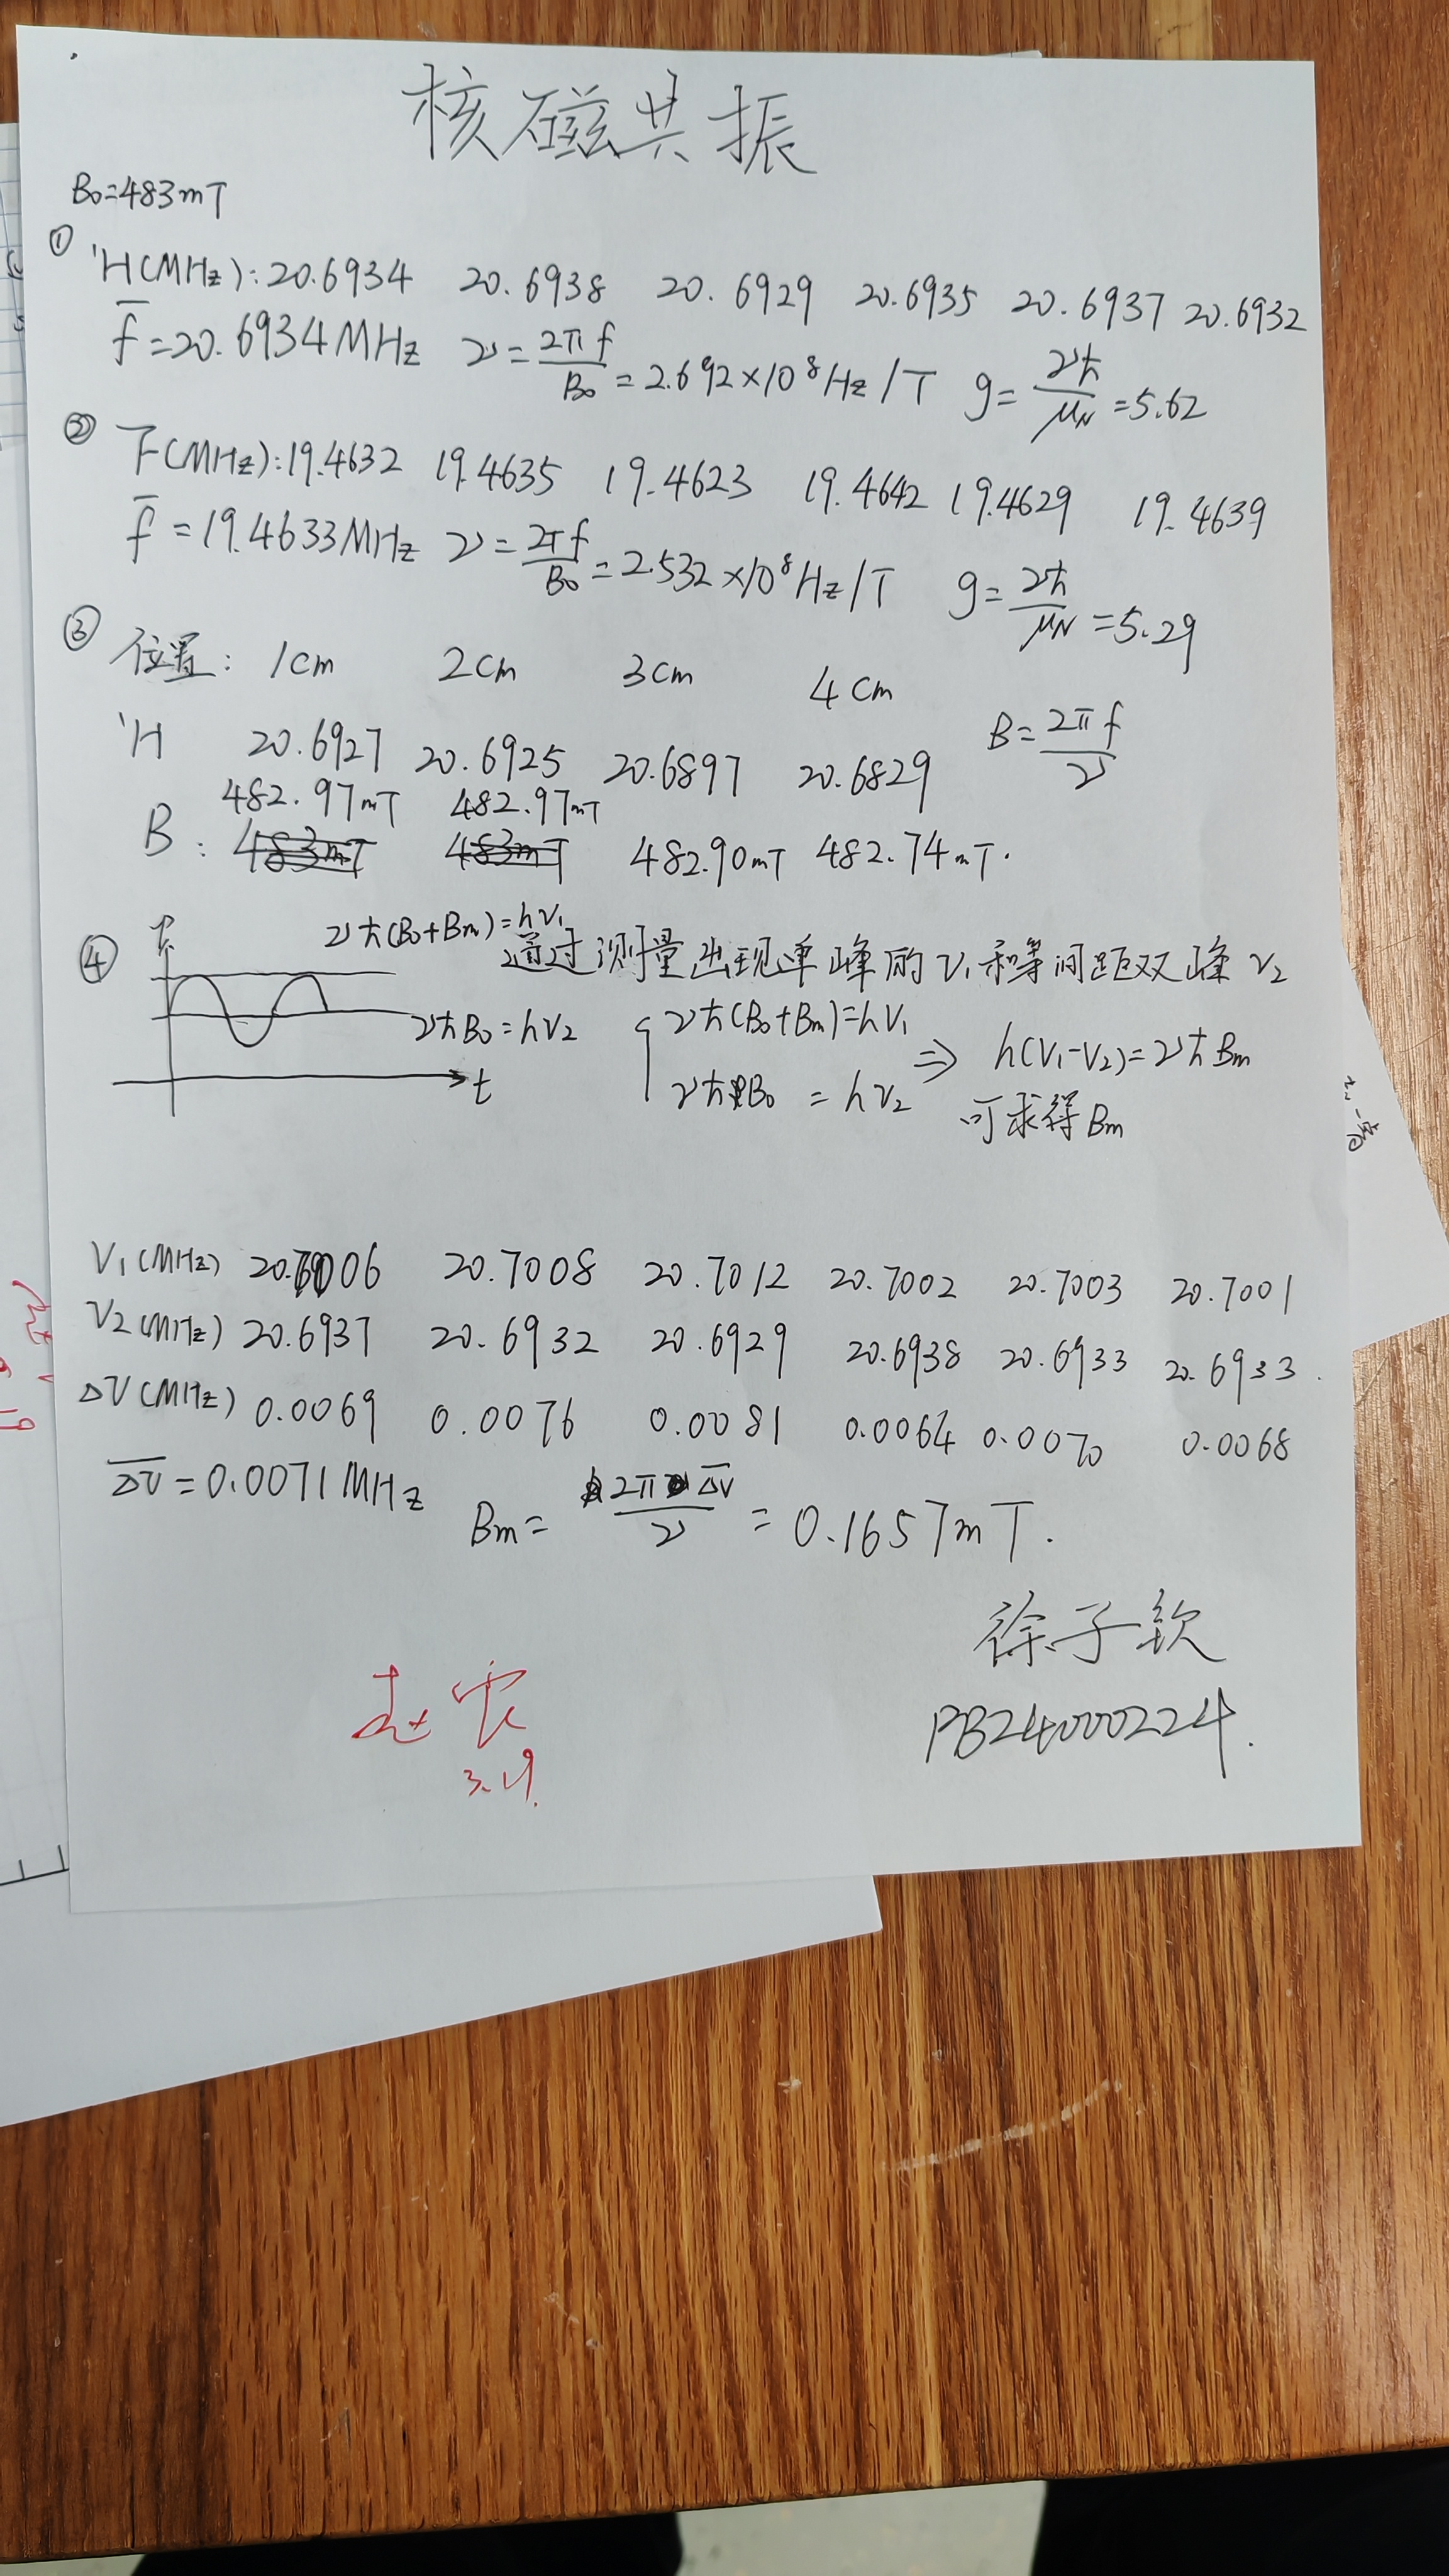
\includegraphics[width=0.72\textwidth,height=0.78\textheight,keepaspectratio]{IMG_20260319_161609.jpg}
    \caption{手写原始数据记录}
\end{figure}

\end{document}